% type de document
\documentclass[11pt]{article}

% Inclusion des packages :
\usepackage{geometry}	% Permet de régler les marges
\usepackage{listings}	% Permet d'inclure des listing de code.
\usepackage[utf8]{inputenc}	% Permet de taper directement les caractères accentués
\usepackage[french]{babel}	% Pries en charge du français.
\usepackage{graphicx}	% Permet d'inclure des images bitmap (jpg,gif,png) ou vectorielles (pdf)


% Instruction poru le package geometry
\geometry{hmargin=1.5cm, vmargin=1.5cm }

% mode de présentation par défaut du package listing
\lstset{language=Java, numbers=left, tabsize=2, frame=single, breaklines=true, numberstyle=\tiny\ttfamily, framexleftmargin=13mm, xleftmargin=12mm}

\author{IDRISSOU SOULER Hamzath}
\title{Rapport de TP - Apprentissage }

% Début du corps du document
\begin{document}

% Provoque l'affichage de l'en-tête :
\maketitle


\section{nombre  voisins}
\subsection{Question 1.2:}
Nous allons dans un premier temps essayer de faire varier le nombre de voisins à regarder afin de pouvoir déterminer correctement le caractère dont on ne connaît que la forme.
Pour cela nous allons avoir besoin de la distance entre deux formes. Les formes étant numérisé dans un tableau de 784 octets, il faudra donc faire le calcul de la distance dans la dimension 784 ! Pour cela nous utiliserons la formule suivante :
Soit $d$ la distance entre un point $\alpha$ et un point $\beta$: \\

$$Z=\sqrt{\sum_{i=0}^{783} ({x_i - y_i})^{2}}$$
où $x_i$ = $i^{e}$ case de la forme connue et $y_i$ = $i^{e}$ case re rechercher.


Une fois, toutes les fonctions utilitaires :génération d'ensemble d'apprentissage et test, recherche des k-plus proches voisins, détermination d'une forme en fonction d'un ensemble de voisins…  des tests seront mis en place afin de déterminer le taux d'erreurs et donc l'efficacité de notre programme.

\begin{lstlisting}
public static void statisticWithKChange(int maxK, int nbModels, int modelSize, int testSize) throws NoMoreDataException {
  List<List<LabelledData>> models = glyphGenerator.getNbGroupGlyph(nbModels, modelSize);
  List<LabelledData> test = glyphGenerator.getNewGroupGlyph(testSize);
  
  double EMT = 0;
  double EMS = 0;
  maxK++;
  
  for(int k = 1; k < maxK; k++) {
    EMT = 0;
    EMS = 0;
    
    for (List<LabelledData> curModel : models) {
      EMS += Utils.erreurMoyenne(curModel, curModel, k);
      EMT += Utils.erreurMoyenne(curModel, test, k);
    }
    EMT /= nbModels;
    EMS /= nbModels;
    System.out.println(k + "\t" + EMT + "\t" + EMS);
  }
}
\end{lstlisting}


Resultat figure \ref{r1}.

\begin{figure}[H]
\center{
	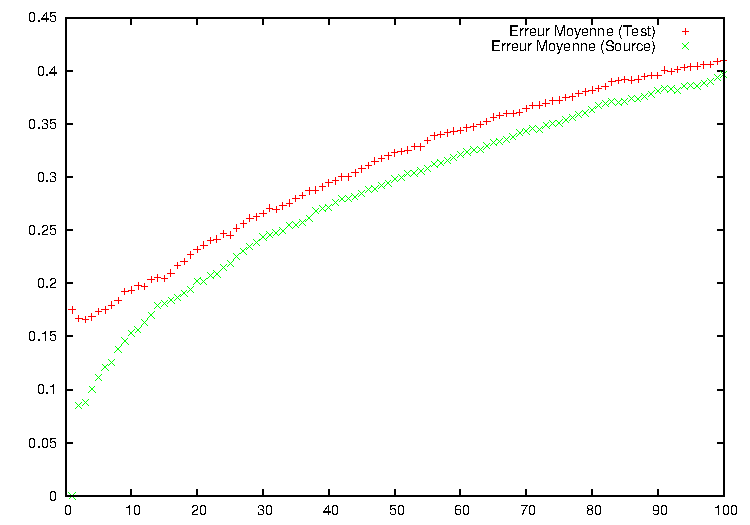
\includegraphics[scale=1]{r1.pdf}
}
\caption{Résultat avec variation k\label{r1}}	% Legende + étiquette
\end{figure}

 plus k devient grand, plus le taux d'erreurs est elevé que cela soit sur l'ensemble de test ou sur l'ensemble sur les ensembles sources. On remarque aussi qu'il y a un point particulier avec k = 3 où le taux d'erreurs est minimale pour l'ensemble de test. 

\section{taille d'ensemble d'apprentissage}
varions la taille des ensembles d'apprentissage pour voir si cela a un impact sur le taux d'erreurs. On fixera k, le nombre de voisins recherchés, à 3 comme nous l'avons vu avant cette valeur était la meilleur. On se propose de réaliser cette fois ce programme qui est très semblable au précédent :

\begin{lstlisting}
public static void statisticWithModelChange(int k, int nbModels, int minModelSize, int maxModelSize, int testSize) throws NoMoreDataException {
  if (minModelSize > maxModelSize) {
    throw new IllegalArgumentException("Min > Max");
  }
  List<LabelledData> test = glyphGenerator.getNewGroupGlyph(testSize);
  
  double EMT = 0;
  double EMS = 0;
  
  for(int i = minModelSize; i <= maxModelSize; i++) {
    EMT = 0;
    EMS = 0;
    
    List<List<LabelledData>> models = glyphGenerator.getNbGroupGlyphWithoutRetail(nbModels, i);
    
    for (List<LabelledData> curModel : models) {
      EMS += Utils.erreurMoyenne(curModel, curModel, k);
      EMT += Utils.erreurMoyenne(curModel, test, k);
    }
    EMT /= nbModels;
    EMS /= nbModels;
    System.out.println(i + "\t" + EMT + "\t" + EMS);
  }
}
\end{lstlisting}

résultats de la Figure \ref{r2}.

\begin{figure}[H]
\center{
	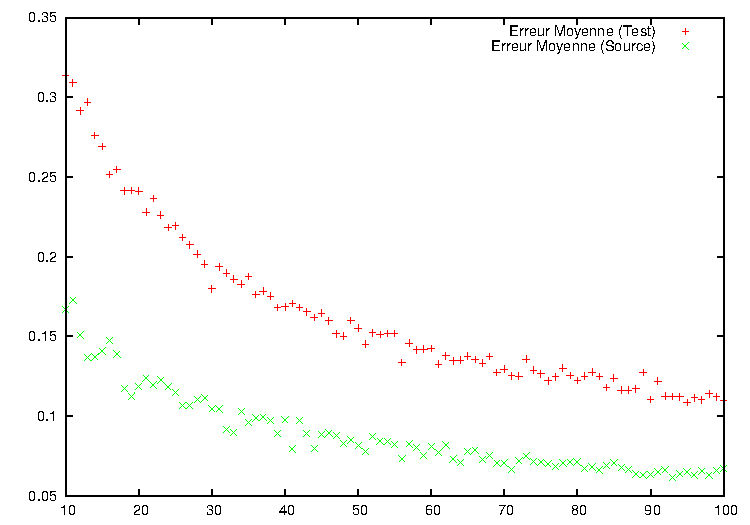
\includegraphics[scale=1]{r2.pdf}
}
\caption{Résultat du test avec  variation de  la taille des ensembles d'apprentisage\label{r2}}	% Legende + étiquette
\end{figure}

remarque :le taux d'erreurs, peut importe sur les ensembles d'apprentissage ou  les données de test, décroit avec un ensemble plus grand de données de base. 

\section{Problème du nombre de voisins égaux}

Une  solution, a ce problème consisterai à faire la somme des distances pour les caractères A et pour les caractères B, ensuite on compare les deux sommes et l'on si ce sont globalement les A ou les B qui sont les plus proches.

\section{conclusion}
Nous avons donc appris au cours de ce TP que pour réduire le taux d'erreurs sur notre programme de reconnaissance de caractères (formes). Il fallait tout d'abord trouver un k optimal pour nous on a trouvé 3.  Enfin nous avons vu que nous pouvions encore améliorer notre programme lors de conflits pour le choix du caractère représenté par la forme que nous recherchons.

\end{document}
